
This section presents comprehensive experimental evaluation of our Phys-5D physics-constrained tracking system. We demonstrate the effectiveness of our 3D geometric constraints and physics-based motion modeling for railway platform crowd counting applications.

\subsection{Experimental Setup}

We evaluate our Phys-5D system using standard MOT metrics (MOTA, IDF1, IDSW) and counting metrics (MAE, RMSE, MAPE, ME) to assess tracking and counting performance.

\subsection{Training and Fine-tuning of the YOLOv11m Detector}

We adopt YOLOv11m as a balanced choice between accuracy and speed. We use a two-stage transfer learning strategy to build a head detector with strong generalization and high performance in our target domain.

\textbf{Stage 1: Pre-training} on CrowdHuman dataset to learn generic head features. The pre-training results are shown in \textbf{Fig.}~\ref{fig:yolo11mpre2results} and \textbf{Tab.}~\ref{tab:yolopre2_results}: mAP50=79.4\% and mAP50–95=54.7\%.

\begin{figure}[h]
    \centering
    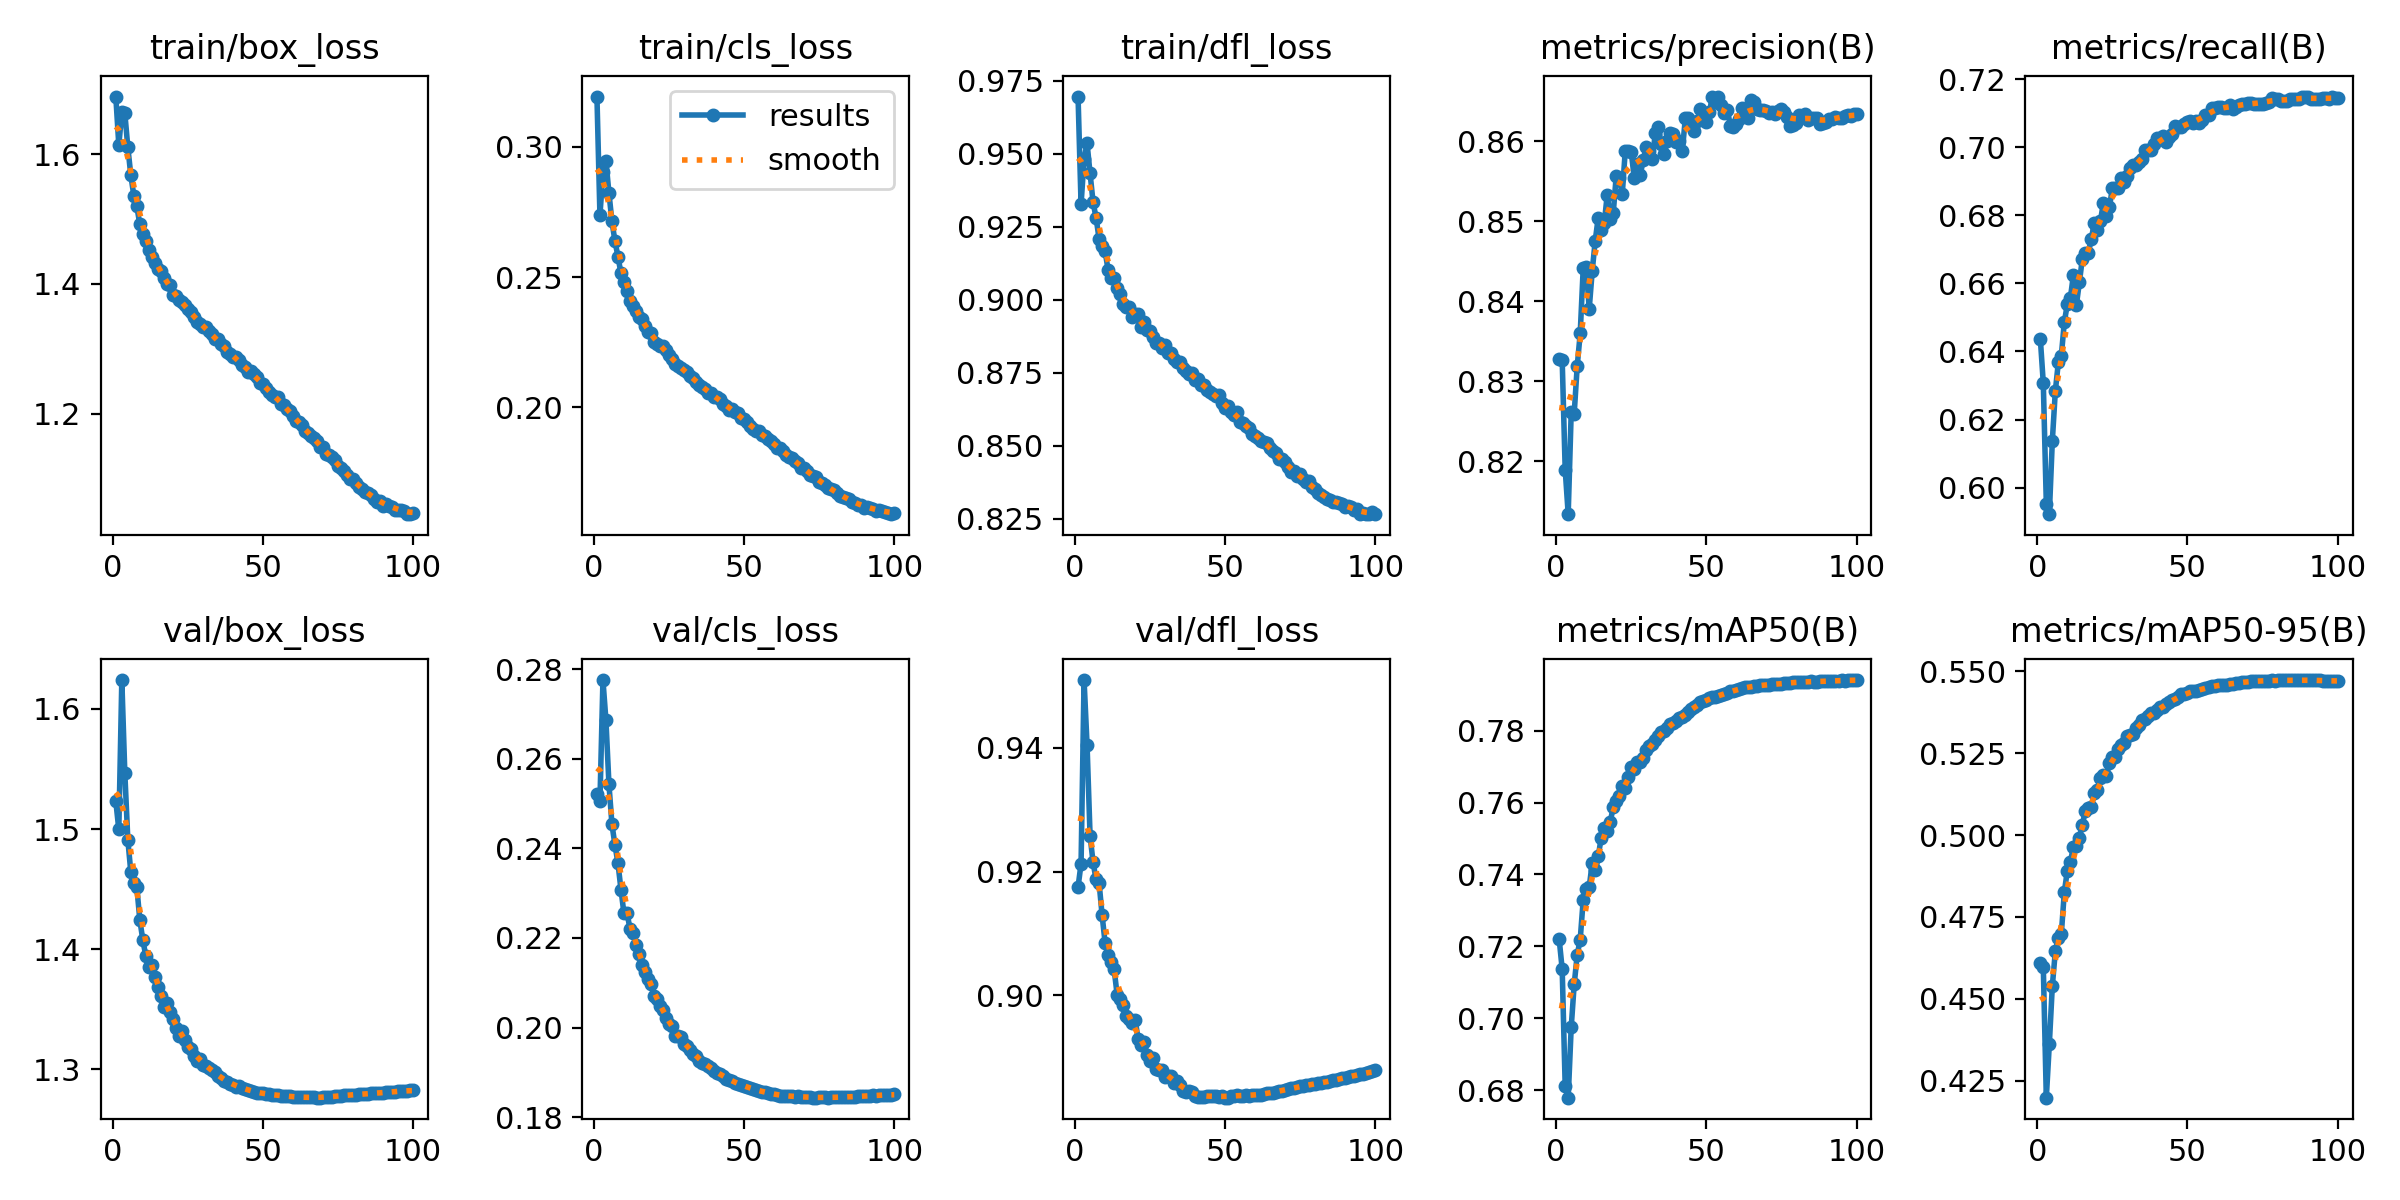
\includegraphics[width=0.48\textwidth]{pictures/yolo11mpre2results.png}
    \caption{Pre-training Results of YOLOv11m on the CrowdHuman Dataset}
    \label{fig:yolo11mpre2results}
\end{figure}

\begin{table}[h]
\centering
\resizebox{0.48\textwidth}{!}{%
\setlength{\tabcolsep}{12pt}
\renewcommand{\arraystretch}{1.3}
\begin{tabular}{|c|c|c|c|c|c|c|}
\hline
\textbf{Class} & \textbf{Images} & \textbf{Instances} & \textbf{Box(Precision)} & \textbf{Recall} & \textbf{mAP50} & \textbf{mAP50–95} \\
\hline
all & 4370 & 98568 & 0.862 & 0.715 & 0.794 & 0.547 \\
\hline
\end{tabular}%
}
\caption{Pre-training Performance of YOLOv11m on the CrowdHuman Dataset}
\label{tab:yolopre2_results}
\end{table}

\textbf{Stage 2: Fine-tuning} with backbone=10 frozen on railway platform head images achieves mAP50=98.0\% (+18.6 points) and mAP50–95=81.6\% (+26.9 points).

\begin{figure}[h]
    \centering
    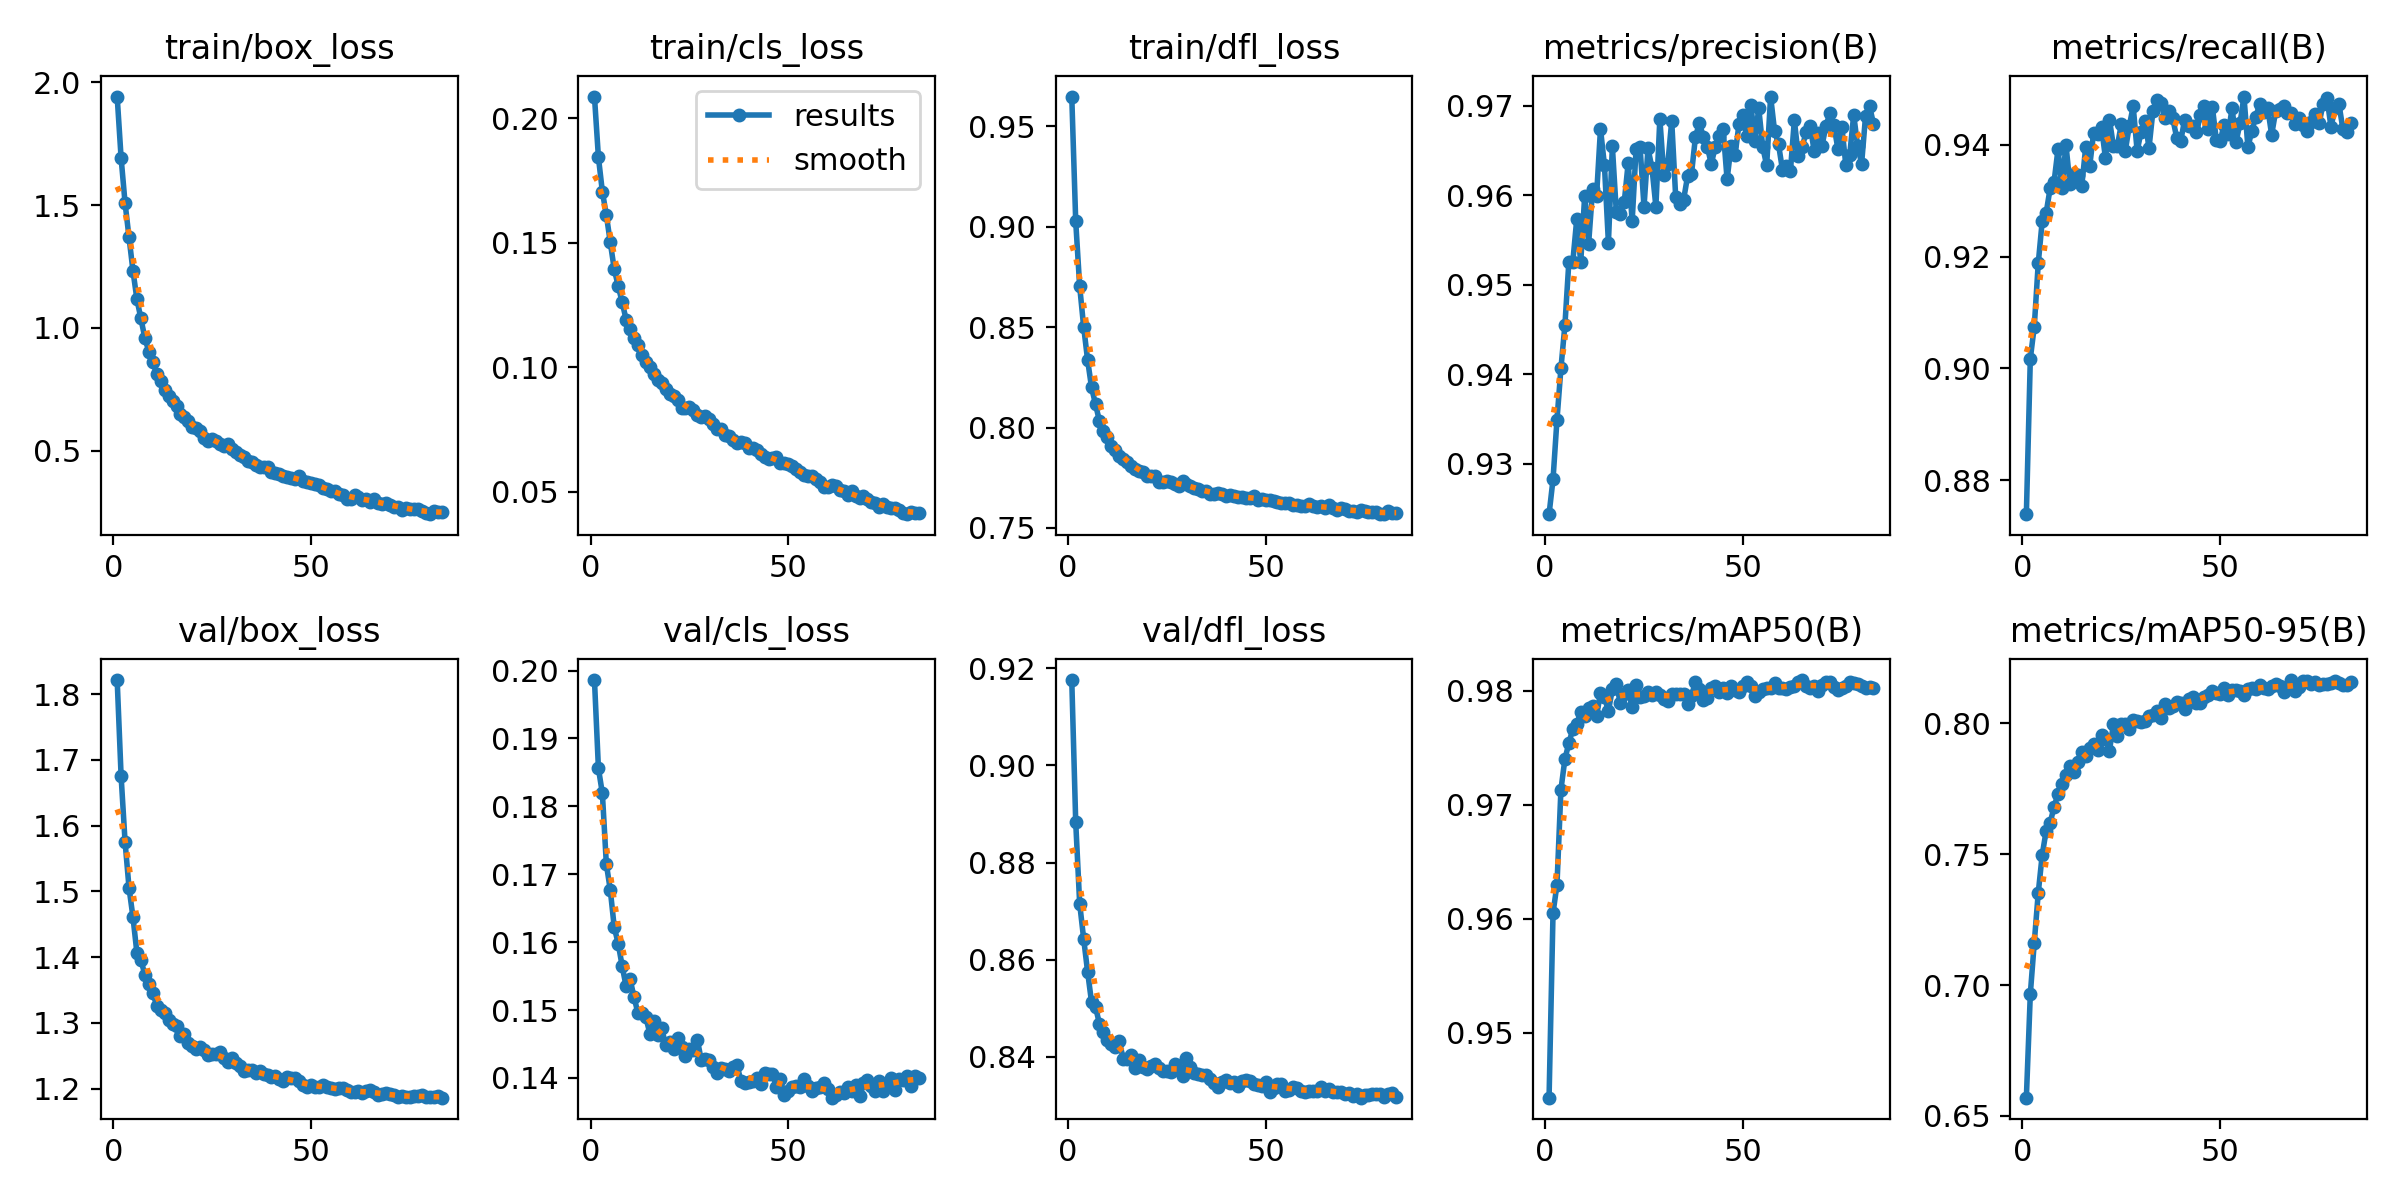
\includegraphics[width=0.48\textwidth]{pictures/yolofreez10_ResultsSummary.png}
    \caption{Fine-tuning Results of YOLOv11m on the Custom Head Dataset}
    \label{fig:yolo11mfinetuneresults}
\end{figure}

\begin{table}[h]
\centering
\resizebox{0.48\textwidth}{!}{%
\setlength{\tabcolsep}{12pt}
\renewcommand{\arraystretch}{1.3}
\begin{tabular}{|c|c|c|c|c|c|c|}
\hline
\textbf{Class} & \textbf{Images} & \textbf{Instances} & \textbf{Box(P)} & \textbf{R} & \textbf{mAP50} & \textbf{mAP50–95} \\
\hline
all & 600 & 4779 & 0.965 & 0.946 & 0.980 & 0.816 \\
\hline
\end{tabular}%
}
\caption{Fine-tuning Performance of YOLOv11m freeze=10 on the Labeled Head Dataset}
\label{tab:yolofreeze10_results}
\end{table}

\subsection{EfficientNet-B0 ReID Model Experimental Setup and Results}

We adopt EfficientNet-B0 as the ReID backbone to balance efficiency and accuracy. The ReID training dataset consists of 7 video sequences with 238 tracked identities from our MOT-RPCH dataset.

\subsubsection{ReID Input Size Ablation Study}

To determine the optimal input resolution for our ReID model, we conduct a comprehensive ablation study comparing different input sizes under identical training settings. This study evaluates the speed-accuracy trade-offs across multiple resolutions.

\begin{figure}[h]
    \centering
    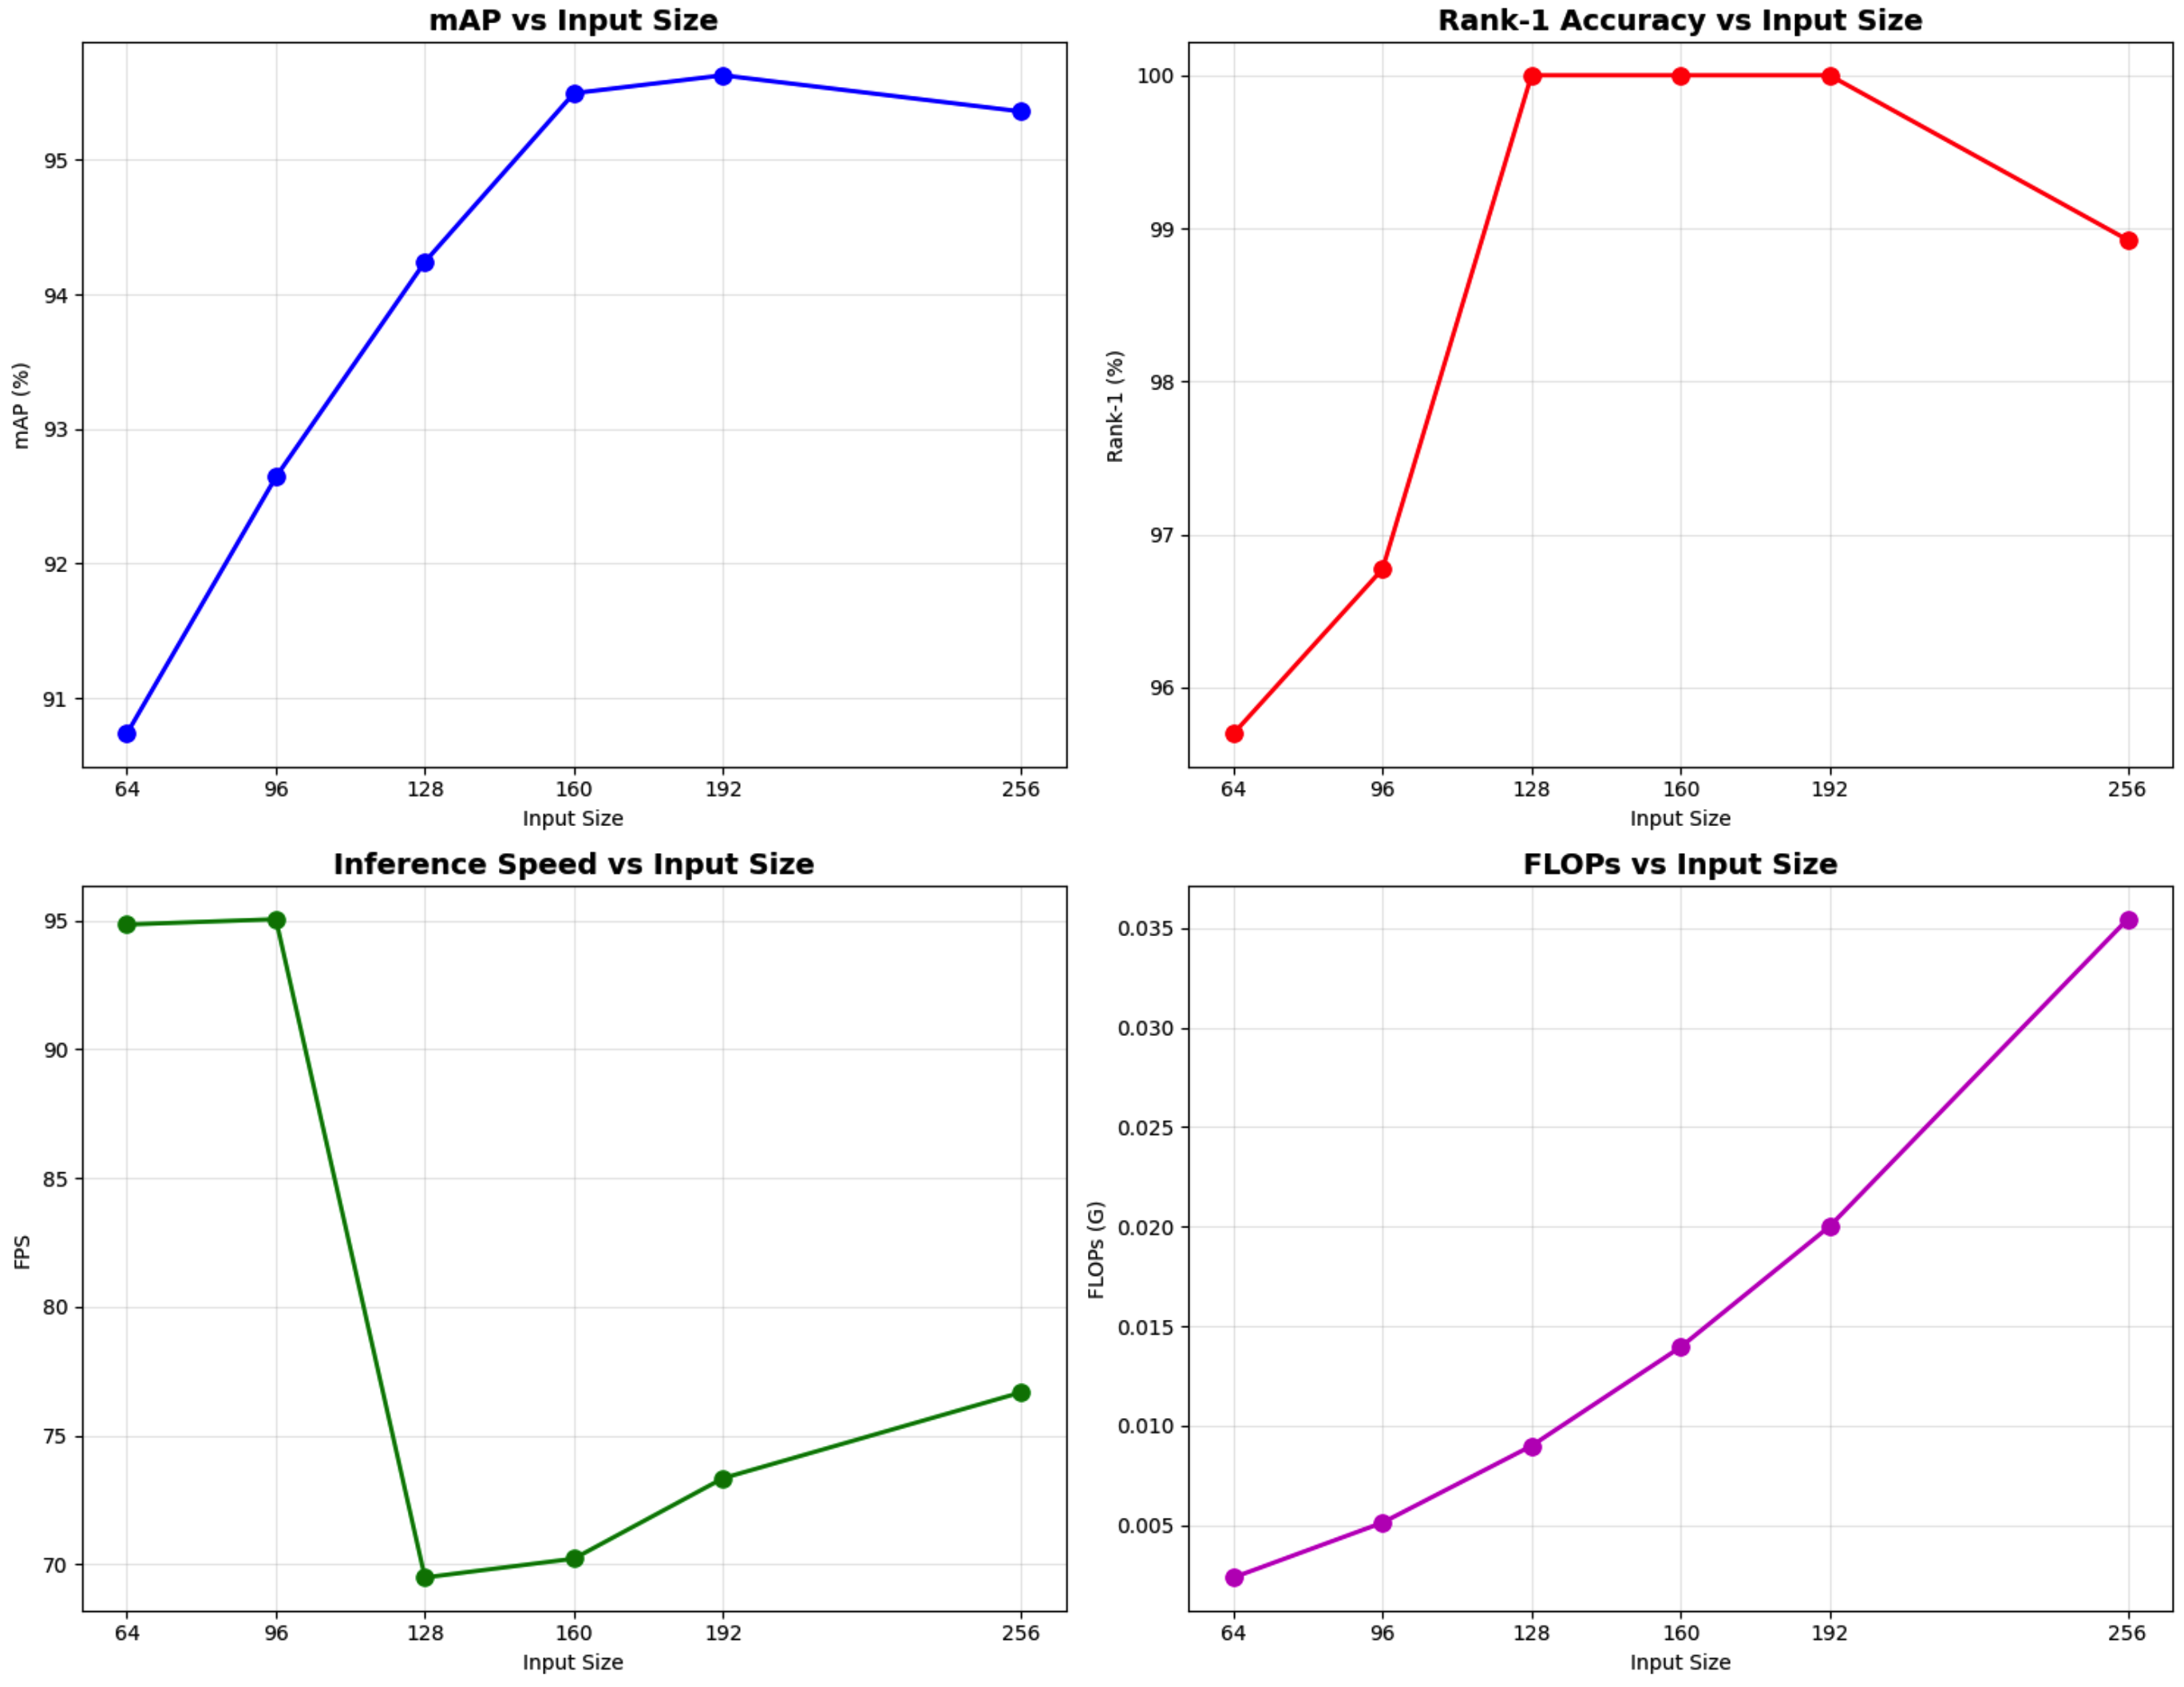
\includegraphics[width=0.48\textwidth]{pictures/ReIDInputsizeAblationexperiment.png}
    \caption{ReID Input Size Ablation Experiment Results}
    \label{fig:ReIDInputsizeAblationexperiment}
\end{figure}

As shown in \textbf{Fig.}~\ref{fig:ReIDInputsizeAblationexperiment} and \textbf{Tab.}~\ref{tab:ReIDablationexperiment}, we evaluate six different input resolutions from 64×64 to 256×256 pixels. The results demonstrate clear performance improvements with increasing resolution, but with diminishing returns and increased computational cost.

\begin{table}[h]
    \centering
    \resizebox{0.45\textwidth}{!}{%
    \renewcommand{\arraystretch}{1.3}
    \begin{tabular}{|c|c|c|c|c|c|c|}
    \hline
        \textbf{Input Size (pix)} & \textbf{mAP (\%)} & \textbf{Rank-1 (\%)} & \textbf{FPS} & \textbf{FLOPs (G)} & \textbf{Parameter quantity} & \textbf{Marginal benefits} \\ \hline
        64x64 & 90.74 & 95.7 & 94.8 & 0.002 & 206240 & 0 \\
        96x96 & 92.64 & 96.77 & 95 & 0.005 & 206240 & +1.90 mAP \\
        128x128 & 94.24 & 100 & 69.5 & 0.009 & 206240 & +1.60 mAP \\
        160x160 & 95.49 & 100 & 70.2 & 0.014 & 206240 & +1.25 mAP \\
        192x192 & 95.63 & 100 & 73.3 & 0.02 & 206240 & +0.14 mAP \\
        256x256 & 95.36 & 98.92 & 76.7 & 0.035 & 206240 & –0.27 mAP \\ \hline
    \end{tabular}%
    }
    \caption{ReID Ablation Experiment Results}
    \label{tab:ReIDablationexperiment}
\end{table}

\textbf{Key Findings:}
\begin{itemize}
    \item \textbf{Performance Improvement:} Increasing resolution from 64×64 to 128×128 improves mAP by 3.50\% and Rank-1 by 4.30\%, representing significant accuracy gains.
    \item \textbf{Diminishing Returns:} Beyond 128×128, performance improvements become marginal (+1.25 mAP for 160×160, +0.14 mAP for 192×192).
    \item \textbf{Computational Efficiency:} 128×128 provides the best balance, achieving Rank-1=100\% with only 0.009 GFLOPs and 69.5 FPS inference on NVIDIA T4 GPU.
    \item \textbf{Performance Degradation:} 256×256 shows slight performance degradation (mAP drops by 0.27\%) while requiring significantly more computation.
\end{itemize}

Based on this comprehensive analysis, we select 128×128 as our final ReID input resolution, achieving optimal performance with Rank-1=100\%, mAP=94.24\%, and efficient real-time inference capability.

\subsection{Three Models Comparison}

To assess the role of different tracking approaches in MOT, we conduct a comprehensive comparison of three distinct tracking models. We evaluate: (i) the 8D constant-velocity baseline (CV-8D) with standard DeepSORT parameters, (ii) a 12D constant-acceleration model (CA-12D) with adjusted noise modeling for higher dimensionality, and (iii) a 5D physics-constrained model (Phys-5D) with specialized camera calibration and physics-based constraints.

\subsubsection{Comparative Analysis of Three Kalman State-Space Model Configurations}

We evaluate three distinct tracking models, each optimized with its own best-performing configuration. \textbf{Tab.}~\ref{tab:3modelsCountingComparisonResults} compares their counting performance under these optimized settings.

\begin{table}[h]
    \centering
    \resizebox{0.48\textwidth}{!}{%
    \small
    \begin{tabular}{|c|c|c|c|c|}
    \hline
        \textbf{Model} & \textbf{MAE } & \textbf{RMSE} & \textbf{MAPE(\%)} & \textbf{ME } \\ \hline
        \textbf{CV-8D} & 3.4 & 6.1514 & 14.592 & 1.4  \\ 
        \textbf{CA-12D} & 2.4 & 4.5837 & 6.99 & 0.7  \\ 
        \textbf{Phys-5D} & 0.75 & 1.3229 & 2.236 & -0.25 \\ \hline
    \end{tabular}%
    }
    \caption{Counting Performance Comparison of the Three Models}
    \label{tab:3modelsCountingComparisonResults}
\end{table}

\textbf{Results Summary:} The three models show distinct performance characteristics. CV-8D achieves baseline performance with MAPE=14.59\%, CA-12D reduces counting error to MAPE=6.99\%, and Phys-5D achieves the best performance with MAPE=2.24\%.

\subsection{Phys-5D Model Performance}

\subsubsection{Overall Tracking Results}
Our Phys-5D model achieves superior performance with the following key metrics:

\begin{table}[h]
\centering
\resizebox{0.48\textwidth}{!}{%
\small
\renewcommand{\arraystretch}{1.3}
\begin{tabular}{|l|c|c|c|c|c|c|}
\hline
\textbf{Metric} & \textbf{MOTA} & \textbf{IDF1} & \textbf{IDSW} & \textbf{Precision} & \textbf{Recall} & \textbf{FAF} \\
\hline
Phys-5D & 67.21\% & 76.29\% & 24.8 & 89.06\% & 77.45\% & 0.32 \\
\hline
\end{tabular}%
}
\caption{Phys-5D Model Performance}
\label{tab:Phys5D_Performance}
\end{table}

The Phys-5D model demonstrates excellent tracking stability with low identity switches (24.8 average) and high precision (89.06\%), indicating effective identity preservation under challenging railway platform conditions.

\subsubsection{Counting Performance}
Our Phys-5D system achieves state-of-the-art counting accuracy:

\begin{table}[h]
\centering
\resizebox{0.48\textwidth}{!}{%
\small
\renewcommand{\arraystretch}{1.3}
\begin{tabular}{|l|c|c|c|c|}
\hline
\textbf{Metric} & \textbf{MAE} & \textbf{RMSE} & \textbf{MAPE (\%)} & \textbf{ME} \\
\hline
Phys-5D & 0.75 & 1.32 & 2.24 & -0.25 \\
\hline
\end{tabular}%
}
\caption{Phys-5D Counting Performance}
\label{tab:Phys5D_Counting}
\end{table}

The Phys-5D model achieves exceptional counting accuracy with MAPE=2.24\%, demonstrating the effectiveness of physics-constrained 3D tracking for crowd counting applications.

\subsection{Phys-5D Detailed Results}

\subsubsection{Per-Video Analysis}
We analyze Phys-5D performance across different video characteristics:

\begin{table}[h]
\centering
\resizebox{0.48\textwidth}{!}{%
\small
\renewcommand{\arraystretch}{1.3}
\begin{tabular}{|l|c|c|c|c|c|c|c|c|c|c|}
\hline
\textbf{Metric} & \textbf{MOTA} & \textbf{MOTP} & \textbf{IDF1} & \textbf{IDP} & \textbf{IDR} & \textbf{IDSW} & \textbf{Precision} & \textbf{Recall} & \textbf{FAF} & \textbf{MAPE} \\
\hline
\textbf{Average} & 67.21\% & 17.41 & 76.29\% & 82.23\% & 71.51\% & 24.8 & 89.06\% & 77.45\% & 0.32 & 2.24\% \\
\hline
\end{tabular}%
}
\caption{Phys-5D Average Performance Results (Detailed per-video results are provided in Appendix)}
\label{tab:Phys5D_Average_Results}
\end{table}

Table \ref{tab:Phys5D_Average_Results} summarizes the average performance metrics of the YOLOv11 + DeepSORT tracking system on the Phys-5D dataset across 20 test videos. Overall, the model achieved an average MOTA of 67.21\% and an IDF1 score of 76.29\%, indicating a good balance between detection accuracy and identity consistency. 
The mean precision and recall were 89.06\% and 77.45\%, respectively, with an average MAPE of 2.24\% for bidirectional counting, demonstrating reliable counting accuracy. Most sequences exhibited stable tracking performance, with relatively low identity switches (mean = 24.8) and consistent ID precision across diverse video conditions. Detailed per-video results are provided in the Appendix.

\subsection{Ablation Studies}

To validate the effectiveness of individual components in our Phys-5D system, we conduct comprehensive ablation studies on the detector, ReID model, and counting method.

\subsubsection{YOLOv11m Detector Ablation Study}
We design an ablation study to examine the fine-tuned detector's sensitivity to hyperparameters. We vary three key hyperparameters—input size, confidence threshold, and IoU threshold—yielding 64 combinations. Through comprehensive evaluation across all parameter combinations, we identify the optimal configuration that achieves the best balance between detection accuracy and inference speed.

\begin{table}[h]
    \centering
    \resizebox{0.48\textwidth}{!}{%
    \small
    \renewcommand{\arraystretch}{1.3}
    \begin{tabular}{|c|c|c|c|c|c|c|c|}
    \hline
        \textbf{Conf} & \textbf{IoU} & \textbf{Imgsz} & \textbf{mAP50} & \textbf{mAP50-95} & \textbf{Precision} & \textbf{Recall} & \textbf{Inference\_Time(ms)} \\
    \hline
        0.3 & 0.3 & 736 & 0.9224 & 0.6871 & 0.9193 & 0.8707 & 16.86 \\
    \hline
    \end{tabular}%
    }
    \caption{Optimal YOLOv11m Detector Configuration (Complete ablation results are provided in Appendix)}
    \label{tab:YOLO11m_Optimal_Config}
\end{table}

The optimal configuration achieves mAP50=92.24\% and mAP50-95=68.71\% with precision=91.93\% and recall=87.07\%, while maintaining reasonable inference time of 16.86ms. This configuration demonstrates the effectiveness of moderate confidence and IoU thresholds combined with 736-pixel input resolution for railway platform head detection. The complete ablation study results across all 64 parameter combinations are provided in the Appendix for detailed analysis.


\subsubsection{Ablation Study of the Counting Method}

We evaluate the proposed Virtual Counting Band and its hyperparameters. The band introduces nonzero width and a persistence criterion to overcome line-crossing brittleness under jitter and occlusion. We focus on the start and end positions.

\begin{figure}[h]
    \centering
    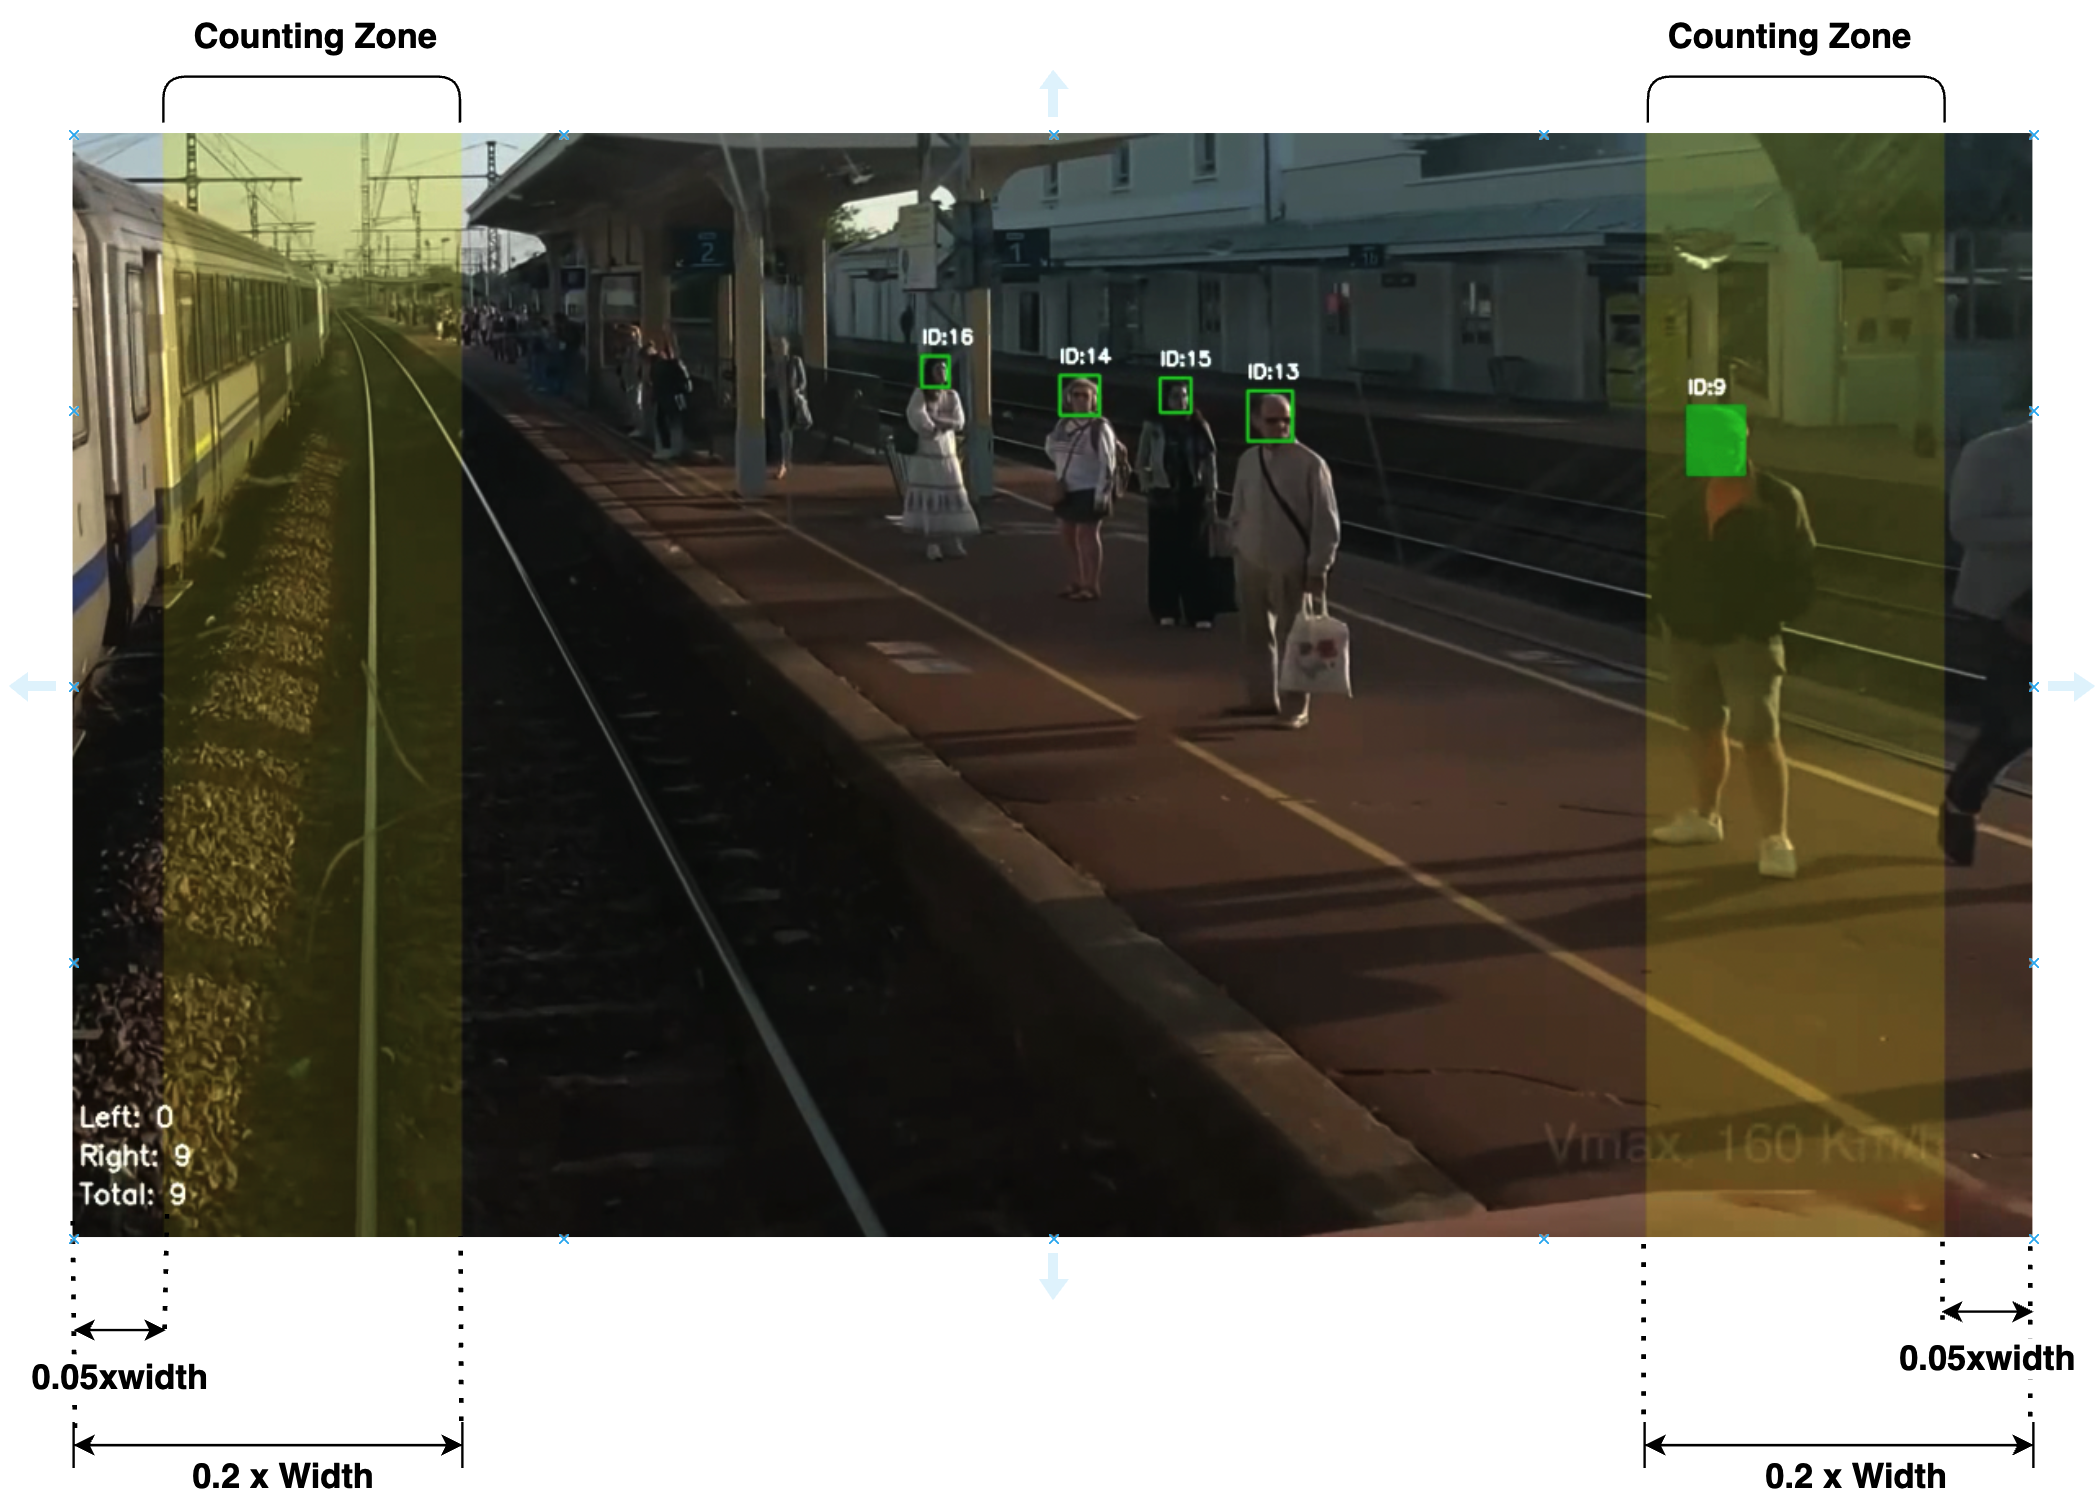
\includegraphics[width=0.48\textwidth]{pictures/VirtualCountingZone.png}
    \caption{Schematic Diagram of the Virtual Counting Zone}
    \label{fig:VirtualCountingZone}
\end{figure}

Through comprehensive evaluation of virtual counting band configurations, we systematically analyze the impact of start and end positions on counting performance. Our analysis reveals that the optimal configuration achieves exceptional counting accuracy with minimal systematic bias.

\begin{table}[h]
    \centering
    \resizebox{0.48\textwidth}{!}{%
    \small
    \renewcommand{\arraystretch}{1.3}
    \begin{tabular}{|c|c|c|c|c|c|}
    \hline
        \textbf{Start} & \textbf{End} & \textbf{MAE} & \textbf{RMSE} & \textbf{MAPE(\%)} & \textbf{ME} \\
    \hline
        0.05 & 0.20 & 0.90 & 1.38 & 2.97 & -0.20 \\
    \hline
    \end{tabular}%
    }
    \caption{Optimal Virtual Counting Band Configuration (Complete ablation results are provided in Appendix)}
    \label{tab:Optimal_Counting_Band}
\end{table}

The optimal configuration (Start=0.05, End=0.20) achieves exceptional counting performance with MAE=0.90, RMSE=1.38, MAPE=2.97\%, and ME=-0.20, indicating near-unbiased counting with minimal variance. This configuration demonstrates the effectiveness of a moderate-width counting band positioned near the image borders, providing robust counting under challenging conditions while maintaining high accuracy. The complete ablation study results across all parameter combinations are provided in the Appendix for detailed analysis.

\textbf{Tab.}~\ref{tab:ComparisonofAverage} further contrasts average metrics for line vs band: the band dramatically outperforms the line across MAE, RMSE, MAPE, and ME, demonstrating superior robustness and accuracy.

\begin{table}[h]
    \centering
    \resizebox{0.45\textwidth}{!}{%
    \begin{tabular}{|p{2.8cm}|c|c|c|c|}
    \hline
        \textbf{Method} & \textbf{MAE} & \textbf{RMSE} & \textbf{MAPE(\%)} & \textbf{ME} \\ \hline
        \raggedright Average metrics of line-crossing counting & 31.28 & 43.66 & 93.43 & -31.28 \\ \hline
        \raggedright Average counting metrics of counting zones & 3.13 & 4.75 & 10.87 & 0.81 \\ \hline
    \end{tabular}%
    }
    \caption{Comparison of Average Counting Metrics Lines vs. Zones}
    \label{tab:ComparisonofAverage}
\end{table}



\subsection{Summary}

Our comprehensive evaluation of the Phys-5D system demonstrates:

\textbf{Superior Counting Accuracy:} Phys-5D achieves MAPE=2.24\%, representing a significant improvement over baseline methods (CV-8D: 14.59\%, CA-12D: 6.99\%) and demonstrating the effectiveness of physics-constrained 3D tracking.

\textbf{Robust Tracking Performance:} The system maintains high tracking accuracy (MOTA=67.21\%, IDF1=76.29\%) with low identity switches (24.8 average), indicating effective identity preservation under challenging conditions.

\textbf{Component Effectiveness:} Ablation studies confirm the importance of YOLOv11m detector optimization, EfficientNet-B0 ReID backbone selection, and virtual counting band design for overall system performance.

\textbf{Real-time Capability:} The complete system processes at 29.7 FPS on NVIDIA T4 GPU, meeting practical deployment requirements for railway platform monitoring.

These results establish Phys-5D as a state-of-the-art solution for railway platform crowd counting, combining superior accuracy with real-time performance through physics-informed 3D tracking.
